\chapter{Analisis}
\label{chap:analisis}

\section{Analisis KIRI}
\label{sec:analisiskiri}
Pada halaman utama KIRI (dapat dilihat pada gambar \ref{fig:3_KIRI_main}), terdapat beberapa bagian yaitu:

\begin{figure}[H]
	\centering
	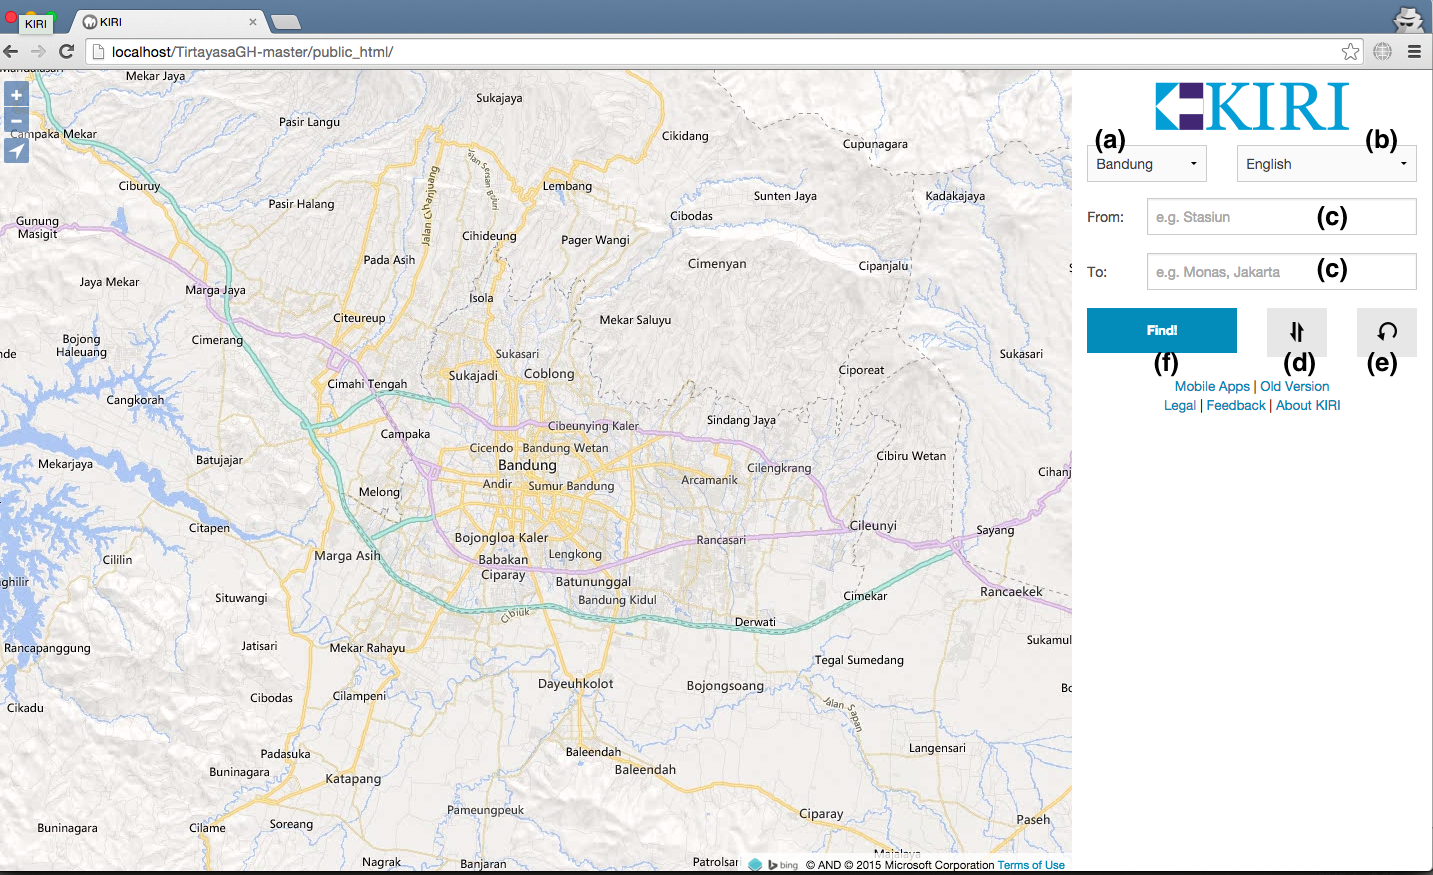
\includegraphics[scale=0.3]{Gambar/KIRI-main}
	\caption{Halaman Utama KIRI} 
	\label{fig:3_KIRI_main}
\end{figure}

\begin{enumerate}
	\item \textbf{Peta}, berfungsi untuk menampilkan peta pada pengguna berdasarkan kota pengguna dan juga menentukan tempat asal dan tujuan pengguna dengan melakukan klik pada peta.
	\item \textbf{Form Samping},
	Form yang terdapat pada halaman utama KIRI terdiri dari:
		\begin{enumerate}
			\item \textbf{Dropdown Menu Kota}, pengguna dapat memilih kota yang dituju (Gambar \ref{fig:3_KIRI_drop_kota}).
			\begin{figure}[H]
				\centering
				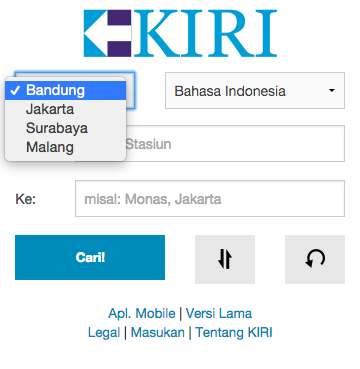
\includegraphics[scale=0.5]{Gambar/KIRI-drop-kota}
				\caption{Dropdown Menu Kota pada KIRI} 
				\label{fig:3_KIRI_drop_kota}
			\end{figure}
			
			\item \textbf{Dropdown Menu Bahasa}, pengguna dapat memilih bahasa yang hendak dipakai (Gambar \ref{fig:3_KIRI_drop_bahasa}).
			\begin{figure}[H]
				\centering
				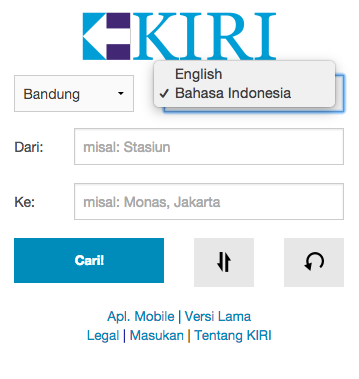
\includegraphics[scale=0.5]{Gambar/KIRI-drop-bahasa}
				\caption{Dropdown Menu Bahasa pada KIRI} 
				\label{fig:3_KIRI_drop_bahasa}
			\end{figure}
			
			\item \textbf{Textfield}, pengguna dapat memasukkan nama tempat asal dan tujuan  (Gambar \ref{fig:3_KIRI_textfield_nama}) atau memasukkan koordinat tempat asal dan tujuan dengan klik pada peta (Gambar \ref{fig:3_KIRI_textfield_koord}).
			\begin{figure}[H]
				\centering
				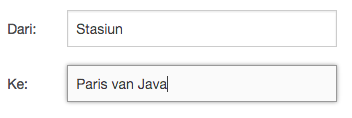
\includegraphics[scale=0.5]{Gambar/KIRI-textfield-nama}
				\caption{Input User(Nama Tempat)} 
				\label{fig:3_KIRI_textfield_nama}
			\end{figure}
			
			\begin{figure}[H]
				\centering
				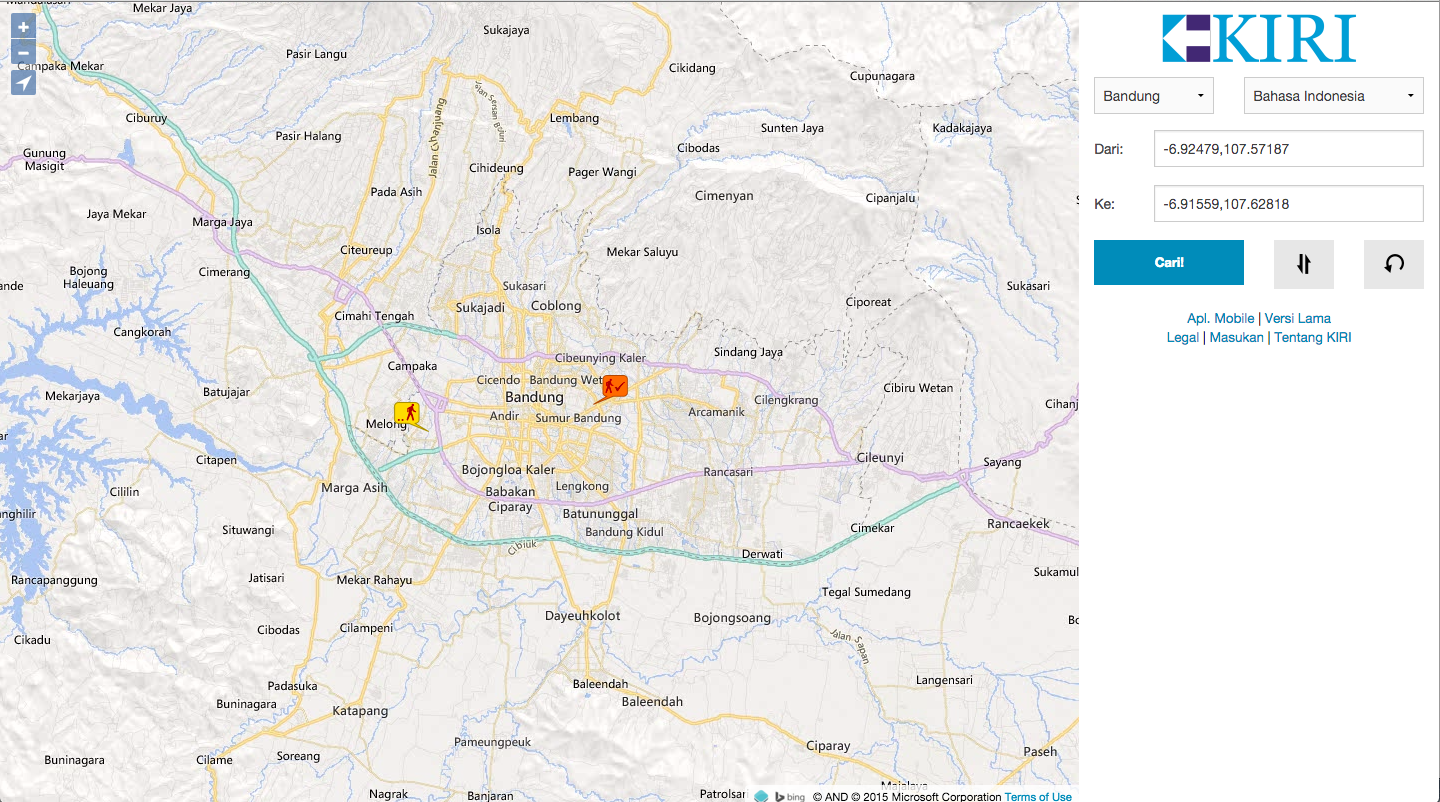
\includegraphics[scale=0.3]{Gambar/KIRI-textfield-koord}
				\caption{Input User(Klik pada peta)} 
				\label{fig:3_KIRI_textfield_koord}
			\end{figure}
		
			\item \textbf{Reset Button}, pengguna dapat melakukan pemilihan tempat dari awal.
			\item \textbf{Swap Button}, pengguna dapat menukar tempat asal dan tujuan.
			\item \textbf{Find Button}, pengguna dapat mencari rute untuk sampai ke tujuan (Gambar \ref{fig:3_KIRI_find}). Pengguna dapat memilih rute alternatif yang sudah disediakan KIRI jika ada (Gambar \ref{fig:3_KIRI_find_alternate}).
			
			\begin{figure}[H]
				\centering
				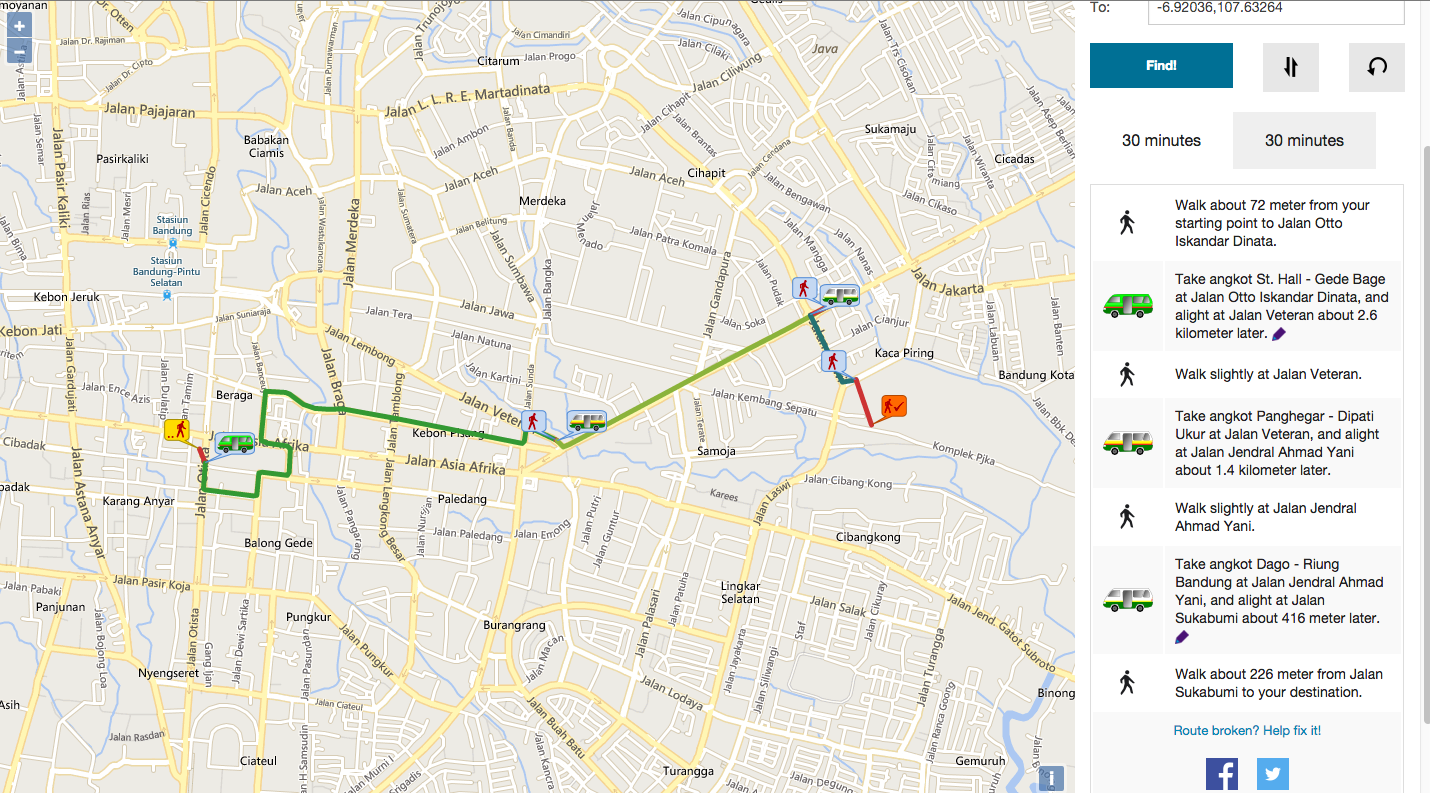
\includegraphics[scale=0.3]{Gambar/KIRI-find}
				\caption{Contoh Pencarian Rute pada KIRI} 
				\label{fig:3_KIRI_find}
			\end{figure}
			
			\begin{figure}[H]
				\centering
				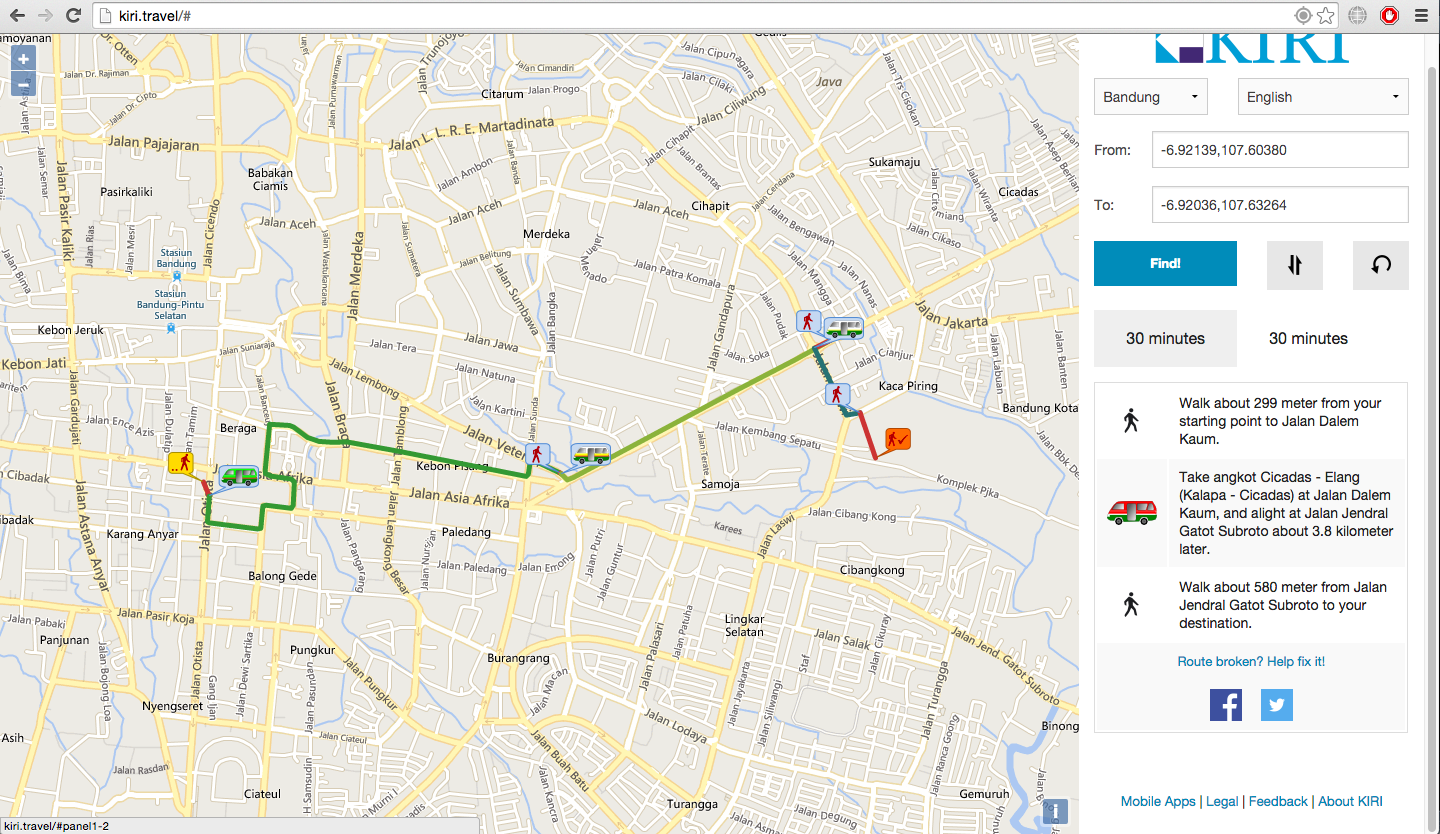
\includegraphics[scale=0.3]{Gambar/KIRI-find-alternate}
				\caption{Contoh Rute Alternatif pada KIRI} 
				\label{fig:3_KIRI_find_alternate}
			\end{figure}
		\end{enumerate}
\end{enumerate}



\section{Perubahan yang dilakukan untuk membuat KIRI dalam Play Framework}
\label{sec:perubahan}
\subsection{Tampilan}
Tampilan pada \play menggunakan format bahasa Scala. Tetapi penggunaan Scala pada \play tidak mengharuskan mahir dalam menggunakan Scala. \play menggunakan Scala tetapi ada ekstensi tambahan lagi yaitu HTML sehingga tidak berbeda jauh dalam penggunaannya dengan HTML biasa hanya dalam Scala, pedeklarasian variabel menggunakan notasi @, sedangkan pada PHP menggunakan notasi \$.


\subsection{JavaScript dan stylesheet}
Penggunaan \textit{stylesheet} dan Javascript pada PHP hanya tinggal memasukkan direktori file yang hendak digunakan, seperti pada kode listing \ref{lst_3_php_js}. Sedangkan pada \play, penggunaan \textit{stylesheet} dan Javascript harus didefinisikan terlebih dahulu pada routes seperti pada kode listing \ref{lst_3_routes}. Pada \cite{playforjava}, untuk akses folder public method yang dipanggil adalah method \verb!at! dan juga tidak disebutkan file mana yang akan diakses, sedangkan pada Play 2.4 method yang dipakai adalah method \verb!versioned! dan menyebutkan file mana yang akan diakses, yaitu file:Asset. Setelah melakukan definisi pada routes, memasukkan stylesheet atau Javascript pada \textit{view} dengan memanggil routes dengan direktori file yang hendak digunakan seperti pada kode listing \ref{lst_3_play_js}. 

\begin{lstlisting}[caption=Penggunaan \textit{stylesheet} dan Javascript pada PHP,label = {lst_3_php_js}]
	<link rel="stylesheet" href="css/styleIndex.css" />
	<script src="foundation/js/vendor/modernizr.js"></script>
\end{lstlisting}

\begin{lstlisting}[caption=Routes untuk penggunaan \textit{stylesheet} dan Javascript,label = {lst_3_routes}]
	GET     /assets/*file               controllers.Assets.versioned(path="/public", file: Asset)
\end{lstlisting}

\begin{lstlisting}[caption=Penggunaan \textit{stylesheet} dan Javascript pada \play,label = {lst_3_play_js}]
	 <link rel="stylesheet" href="@routes.Assets.versioned("css/styleIndex.css")" type="text/css">
	 <script src="@routes.Assets.versioned("foundation/js/vendor/modernizr.js")"></script>
\end{lstlisting}

Untuk mendapatkan elemen View pada JavaScript PHP langsung memanggil \verb!id! tujuan yang ada pada View sebagai parameter, seperti pada kode listing \ref{lst_3_elem_PHP}. Sedangkan pada \play, mendapatkan elemen View pada JavaScript harus menggunakan method document.getElementById dengan parameter berupa \verb!id! tujuan, seperti pada kode listing \ref{lst_3_elem_play}.

\begin{lstlisting}[caption=Mendapatkan elemen View pada JavaScript PHP,label = {lst_3_elem_PHP}]
		$('.tabs').remove();
		$('.tabs-content').remove();
\end{lstlisting}

\begin{lstlisting}[caption=Mendapatkan elemen View pada JavaScript \play,label = {lst_3_elem_play}]
    var tabs = document.getElementById("tabs").remove();
    var tabs_content = document.getElementById("tabs-content").remove();
\end{lstlisting}

\subsection{Internationalization}
Penggunaan Internationalization (i18n) pada PHP dengan cara deklarasi semua variabel yang akan digunakan pada proses i18n terlebih dahulu, misalnya buat file dengan nama tirtayasa\_en.php untuk Bahasa Inggris dan tirtayasa\_id.php untuk Bahasa Indonesia. Pada setiap file tersebut, masukkan \textit{script} PHP untuk menentukan teks yang keluar pada halaman \textit{web} seperti pada kode listing \ref{lst_3_i18n_en} dan kode listing \ref{lst_3_i18n_id}. 

\begin{lstlisting}[caption=Script PHP untuk Bahasa Inggris,label = {lst_3_i18n_en}]
<?php

	$index_about_kiri = "About KIRI";
	$index_apps = "Mobile Apps";
	$index_advanced_ = "Advanced...";
	$index_buyticket = "BUY TICKET";
	$index_connectionerror = 'Connection problem';
?>
\end{lstlisting}


\begin{lstlisting}[caption=Script PHP untuk Bahasa Indonesia,label = {lst_3_i18n_id}]
<?php

	$index_about_kiri = "Tentang KIRI";
	$index_apps = "Apl. Mobile";
	$index_advanced_ = "Lanjut...";
	$index_buyticket = "BUY TICKET";
	$index_connectionerror = 'Gangguan koneksi';
?>
\end{lstlisting}

Penggunaan i18n pada \play hampir sama dengan i18n pada PHP, pertama deklarasi semua variabel yang akan digunakan pada i18n, misal membuat file dengan nama messages.en untuk Bahasa Inggris dan messages.id untuk Bahasa Indonesia. Pada setiap file tersebut, masukkan kunci beserta value untuk untuk menentukan teks yang keluar pada halaman web seperti pada kode listing \ref{lst_3_i18n_play_en} dan kode listing \ref{lst_3_i18n_play_id}.

\begin{lstlisting}[caption=Script \play untuk Bahasa Inggris,label = {lst_3_i18n_play_en}]
from = From:
ph_from = e.g. Stasiun
ph_to = e.g. Monas,Jakarta
find = Find!
to = To:
\end{lstlisting}


\begin{lstlisting}[caption=Script \play untuk Bahasa Indonesia,label = {lst_3_i18n_play_id}]
from = Dari:
ph_from = misal: Stasiun
ph_to = misal: Monas, Jakarta
find = Cari!
to = Ke:
\end{lstlisting}

Setelah itu, masukkan \textit{script} PHP pada \textit{tag} HTML yang ingin diubah saat dilakukan i18n. Adanya \textit{script} PHP pada tag HTML, maka teks akan berubah jika dilakukan i18n seperti pada kode listing \ref{lst_3_i18n_php}. Pada \play, sudah tersedia method untuk i18n, yaitu memanggil method @Messages dengan parameter berupa String yang merupakan kunci dari file messages.LANG. Dengan memanggil method @Messages ini, akan mengganti dengan value pada file messages.LANG seperti pada kode listing \ref{lst_3_i18n_play}.

\begin{lstlisting}[caption=Script PHP untuk Internationalization,label = {lst_3_i18n_php}]
	<label for="startInput" class="inline"><?php print $index_from; ?></label>
	<label for="finishInput" class="inline"><?php print $index_to; ?></label>
	<a href="#" class="small button expand" id="findbutton"><strong><?php print $index_find; ?></strong></a>
\end{lstlisting}

\begin{lstlisting}[caption=Script \play untuk Internationalization,label = {lst_3_i18n_play}]
	<label for="startInput" class="inline">@Messages("from")</label>
	<label for="finishInput" class="inline">@Messages("to")</label>
	<a href="#" class="small button expand" id="findbutton"><strong>@Messages("find")</strong></a>
\end{lstlisting}



\section{Use Case}
\label{sec:usecase}

\begin{figure}[H]
	\centering
	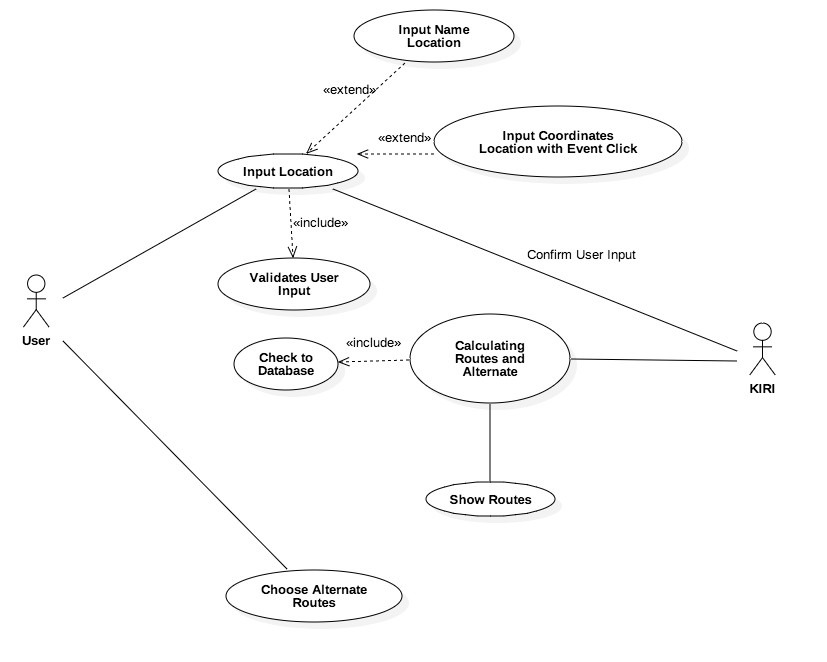
\includegraphics[scale=0.5]{Gambar/usecase}
	\caption{Use Case Diagram KIRI} 
	\label{fig:3_usecase}
\end{figure}

\section{Activity Diagram}
\label{sec:activitydiagram}

\begin{figure}[H]
	\centering
	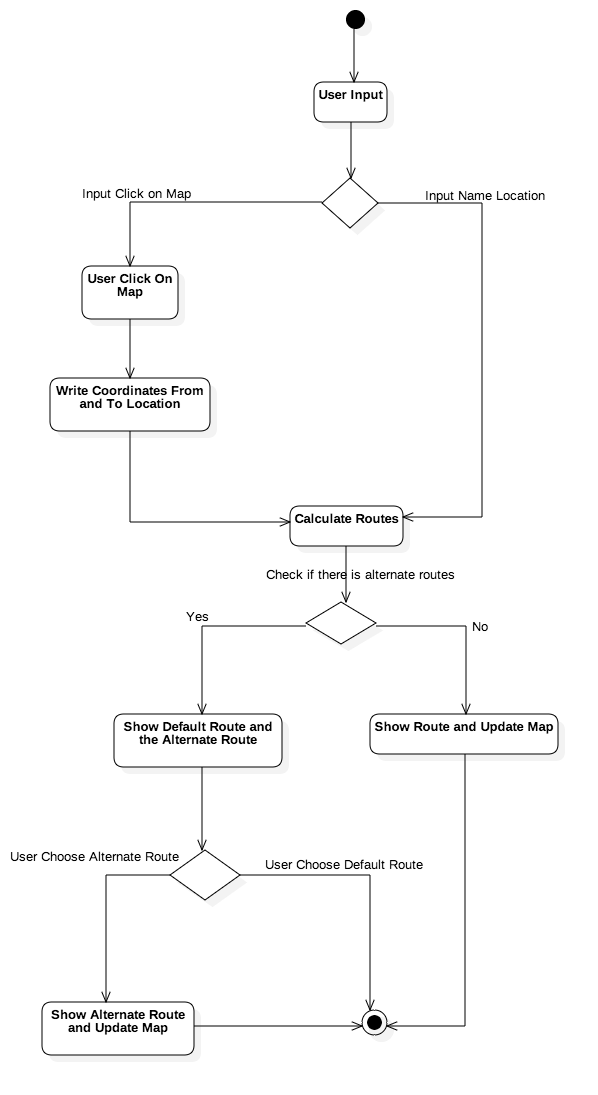
\includegraphics[scale=0.5]{Gambar/activitydiagram}
	\caption{Activity Diagram KIRI} 
	\label{fig:3_activitydiagram}
\end{figure}